\documentclass[10pt,conference]{IEEEtran}
\pagestyle{headings}

\usepackage{cite}
\usepackage{graphicx}
\usepackage{amsmath}
\usepackage{algorithm}
\usepackage{algorithmicx}
\usepackage{algpseudocode}
\usepackage{subfig}
\usepackage{url}
\usepackage{booktabs}
\usepackage{listings}

\renewcommand{\algorithmicrequire}{\textbf{Input:}}
\renewcommand{\algorithmicensure}{\textbf{Output:}}

% correct bad hyphenation here
\hyphenation{op-tical net-works semi-conduc-tor}


\begin{document}
%
% paper title
% can use linebreaks \\ within to get better formatting as desired
\title{ReCapture: A Scalable Testbed for Mobile System Evaluations}

\author{
\IEEEauthorblockN{Jilong Liao}
\IEEEauthorblockA{Department of Electrical Engineering and Computer Science\\
University of Tennessee, Knoxville TN, 37996\\
Email: jliao2@utk.edu}
}

\maketitle


\begin{abstract}
Smartphone related research has been very active in recent years. One important reason is that more and more people tend to use the smart mobile devices which makes it a perfect research tool to study networking, social network and even psychobiology. Besides, people in the system area are also interested in mobile device's performance because it is battery and storage constraint. When researchers want to evaluate their research ideas, e.g. the 3G/4G-LTE network optimization, they have to conduct some large scale evaluations to prove the idea. Unfortunately, this type of evaluation turns out to be a big challenge to the researchers. One obvious reason is that we do not have enough human force and research fundings. So the alternative approach: \emph{small-scale evaluation plus large-scale simulation} becomes the standard methodology in recent year's paper, which definitely is not satisfactory for research. In this paper, we resolve the challenge by adopting the idea of \emph{replay} and \emph{virtualization} which takes the real and easy-to-get usage traces to replay the usage runtime automatically and virtualize the device to scale up the runtime so that the evaluation could be more reliable. We design and implement the system on the Android smartphones, then we evaluate the system through some basic case studies. The results show the system has the ability to reduce the experiment's challenges while make the experiment's result stronger.
\end{abstract}

\IEEEpeerreviewmaketitle

\section{Introduction}\label{sec:introduction}
Mobile devices have been more and more popular in commercial products which gives a user incredible convenience to access Internet services and search the local information. On the other hand, people in research field also realize the significance a mobile device can bring to them. Therefore, more and more research topics have been studied within the smartphones.

For example, researchers are caring about the energy efficiency of a mobile devices like a smartphone or a tablet. They realize the problem is multi-layered which indicates the operating system, network protocol or hardware could have problem. Many literatures have been trying to address this challenges by proposing some techniques and implementing a prototype. Unfortunately, it is difficult for others to repeat the work as they did and get the same results. In other words, the methodology here to evaluate the system is not a complete and reasonable way. Most of them follow a pattern that evaluate the system's performance under one or two smartphones, then using an existing data set to simulate what will happen in practice. However, the simulation itself cannot prove any important conclusion.

The major reason causing this type of incomplete methodology is the reality that we do not have enough devices, time and human force to conduct a large scale experiment. Thereafter, we still have no idea how an idea could work in practice. Even if we have above restriction satisfied, we encounter another problem that it is very hard to control an experiment if we want a person to be involved. For instance, if we want to study the smartphone performance relationship between the user's usage behavior. We may ask the participants to follow some instructions during the experiment. Unfortunately, it is very hard to control the errors between the instructions and the actual use. This could lead to terrible misconclusions in social studies.

In this paper, we propose \emph{ReCapture} which is a large scale automatic testbed for mobile devices. ReCapture is capable of recreating the usage reality from a standard usage trace and a developer is able to plugin any data collection modules to retrieve the desired data. In case that limited physical devices are available, the ReCapture is able to use the virtualization technology to scale up the amount of devices performing an experiments concurrently. 

For a specific experiment, the researcher needs to predefine some user activity log for each devices. Fortunately, many existing data set about a user's usage trace can be the perfect activity log. Those activity logs will trigger each device to follow the same usage behavior on the smartphone. During each usage phase, for instance a user is using Facebook app, the testbed will issue the corresponding screen activity which automatically operate the phone until the usage phase is switched to another app based on the activity log. In this way, a developer can deploy large scale system evaluation based on real user's records instead of simulating the user behavior or relying on the profiling techniques to approximate some metrics like energy consumption.

The rest of the paper is arranged in the following way: Section~\ref{sec:relatedwork} discusses some related work regarding the testbed and virtualization technology in mobile system; Section~\ref{sec:design} describes the system design details and Secion~\ref{sec:implementation} illustrates the system's implementation details; then Section~\ref{sec:evaluation} provides some preliminary performance; finally Section~\ref{sec:conclusion} is our conclusion.

\section{Related Work}\label{sec:relatedwork}
Many research studies have been using smartphones as the testbed or platform to evaluate other information such as environmental information. For example, \cite{lukac2011soundproof} uses smartphone as the platform to monitor wildlife and environment. \cite{jo2013towards} uses the smartphones to build a motion recognition testbed. \cite{heo2010user} analyzes the user demand on the smartphones through a virtual phone environment. However, ReCapture is different from those research because ReCapture is concentrated on the testbed for smartphone related system evaluation. It provides a general testbed for the developers to validate the ideas which could potentially improve the performance on the smartphones or to collect data and study the behaviors in a large scale flavor.

On the other hand, the virtualization technology has improved a lot in the data center which provides the core technology for cloud computing. The virtualization techniques are extremely challenging in mobile environment because of the hardware limitations of the smartphones. \cite{andrus2011cells} implements a virtual mobile phone architecture that could run several virtual phones on the same physical devices. \cite{acharya2009phone} is another approach to achieve the virtualization through the microkernel hypervisor. ReCapture relies on these virtualization technology to scale up the testbed within the limited number of smartphones.

\section{ReCapture Design}\label{sec:design}
The ultimate goal of ReCapture is to give a researcher or developer the capability to run a large scale evaluation about smartphones automatically. Therefore, the design of ReCapture needs the following criterion.
\begin{itemize}
\item Generalness. ReCapture should provide the simple and unified interface for the researches or developers that whatever they want to evaluate on this testbed, they can use the same tool and the same APIs.
\item Flexibility. It requires ReCapture to give the chance for the testbed's input, execution pattern and performance monitoring.
\end{itemize}

\subsection{Core System}
Fig.~\ref{fig:big} shows the big picture of ReCapture. As we can see, we have a central master to organize and schedule testbed and the mobile devices are the testbed to automatically execute the activity log. The central master will load the existing activity log for each device, once the smartphone receive the log activity completely it starts executing the activity script one by one. After the smartphone pull an app in the foreground screen, the central master will be informed which the central master will start sending screen actions to the corresponding smartphone. The screen action script is flexible and can be defined by the developers themselves.

\begin{figure}
\centering
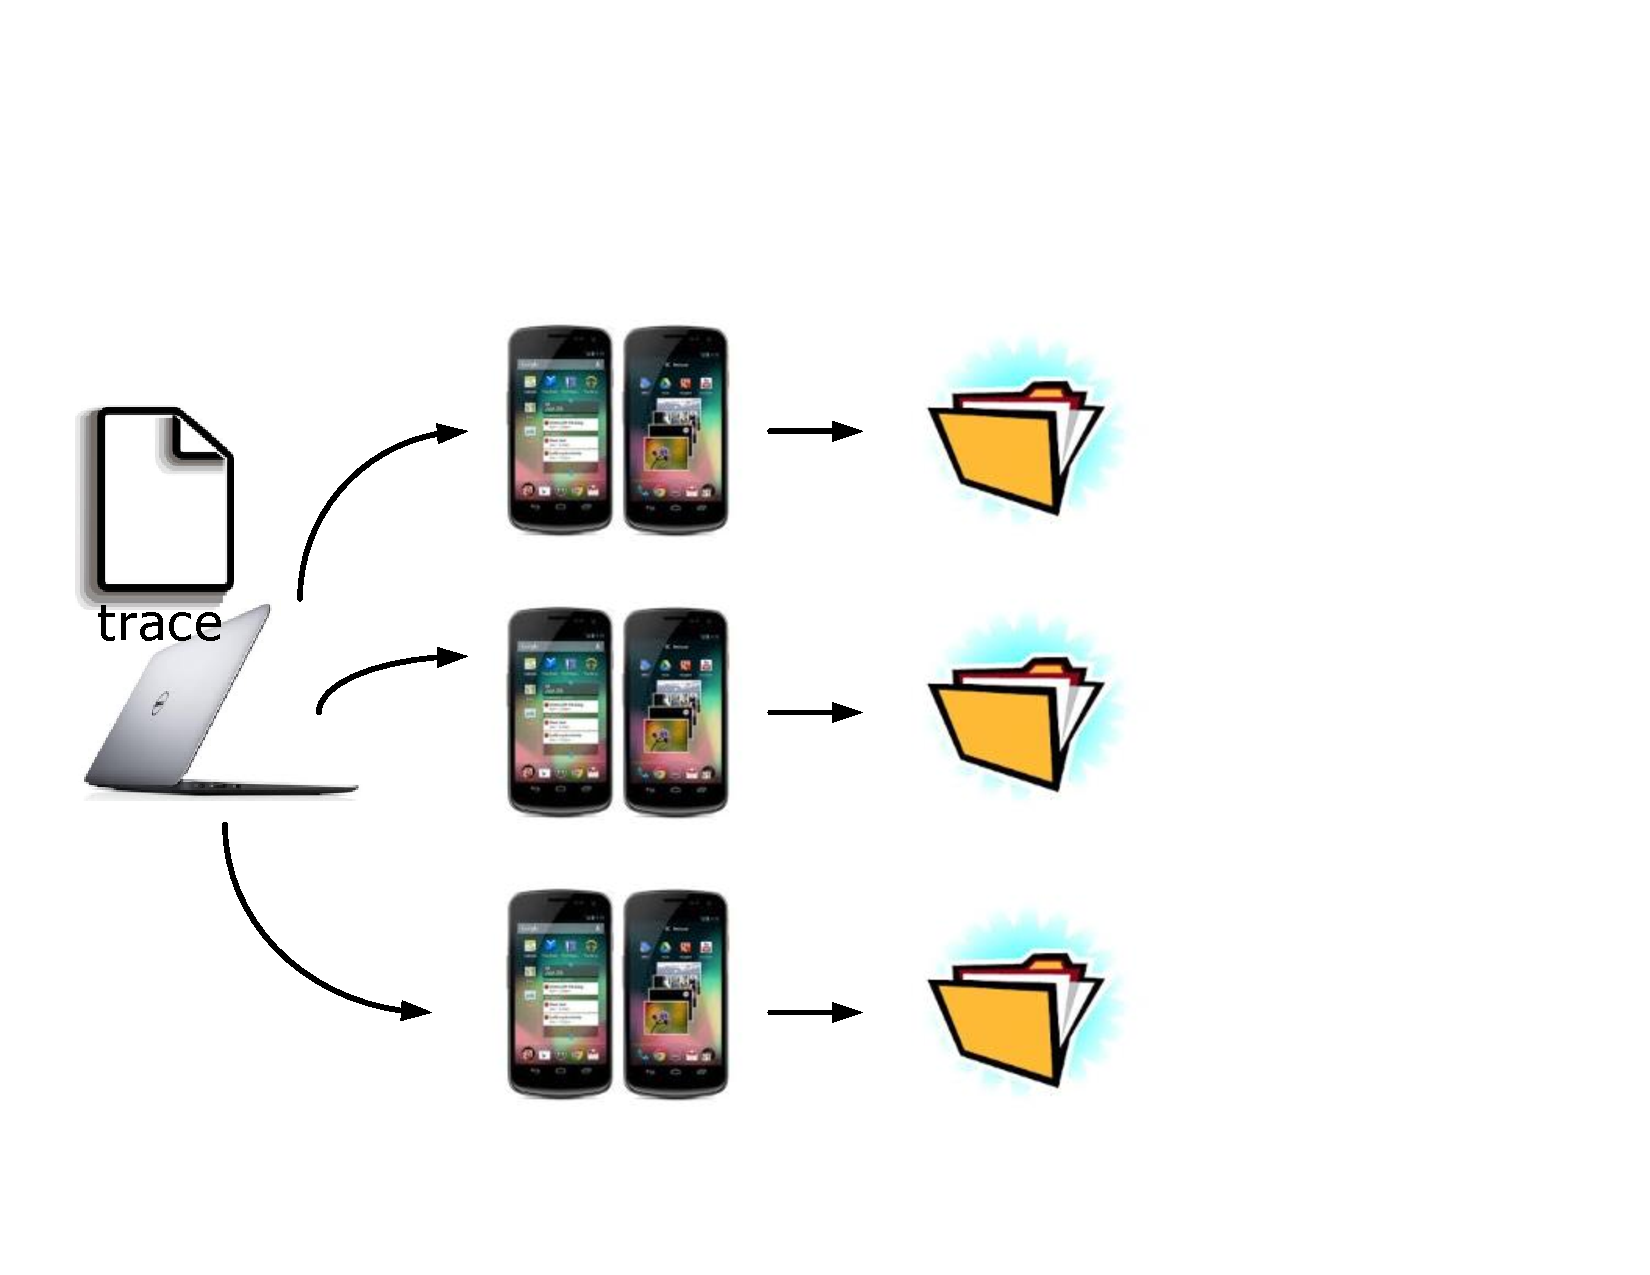
\includegraphics[width=0.45\textwidth]{figures/big-picture.pdf}
\caption{The Big Picture of ReCapture}
\label{fig:big}
\end{figure}

The system architecture is shown in Fig.~\ref{fig:sys}. As is shown, two separate parts are in the system's core architecture: device side and central master side. In the device side, two lightweight components support the runtime environment of the testbed. One is the \emph{scheduler} and the other is \emph{app trigger}. The scheduler takes the activity log (or data trace) received from the central master, then it arranges the execution sequence based on the activity log. For each of the activity event, it starts an app trigger which brings the dedicated app into the screen front. As soon as the the the app is running, the scheduler will send a message to the central master, which will start issuing the screen actions to the device.

Besides the major components, the performance monitor module is presented as a plugin which is flexible to be added and removed. For example, if the developer is interested in the energy consumption of the operating system, he can plugin the energy profiling module into this component. We do not provide identical performance monitoring module inside the ReCapture's framework because 1) we do not want to restrict the extendibility of the system by hard-code everything; 2) we do not want to waste the operating system's resource if the developer is not interested in some monitor like dynamic CPU cost.

On the other hand, the central master have three important modules: synchronization, touch modeling and touch injection. The synchronization module is used to listen the scheduler's commands so that the correct screen actions can be issued. In fact, different app has different usage pattern, so it is important to differentiate among them and model various screen events. Then the screen modeling is the place to model an app's usage action. Normally, a developer can define a series screen actions, this module will go ahead and load the scripts. After the screen action is defined, the touch injector will send the screen actions to the device continuously until the next activity event comes.

\begin{figure}
\centering
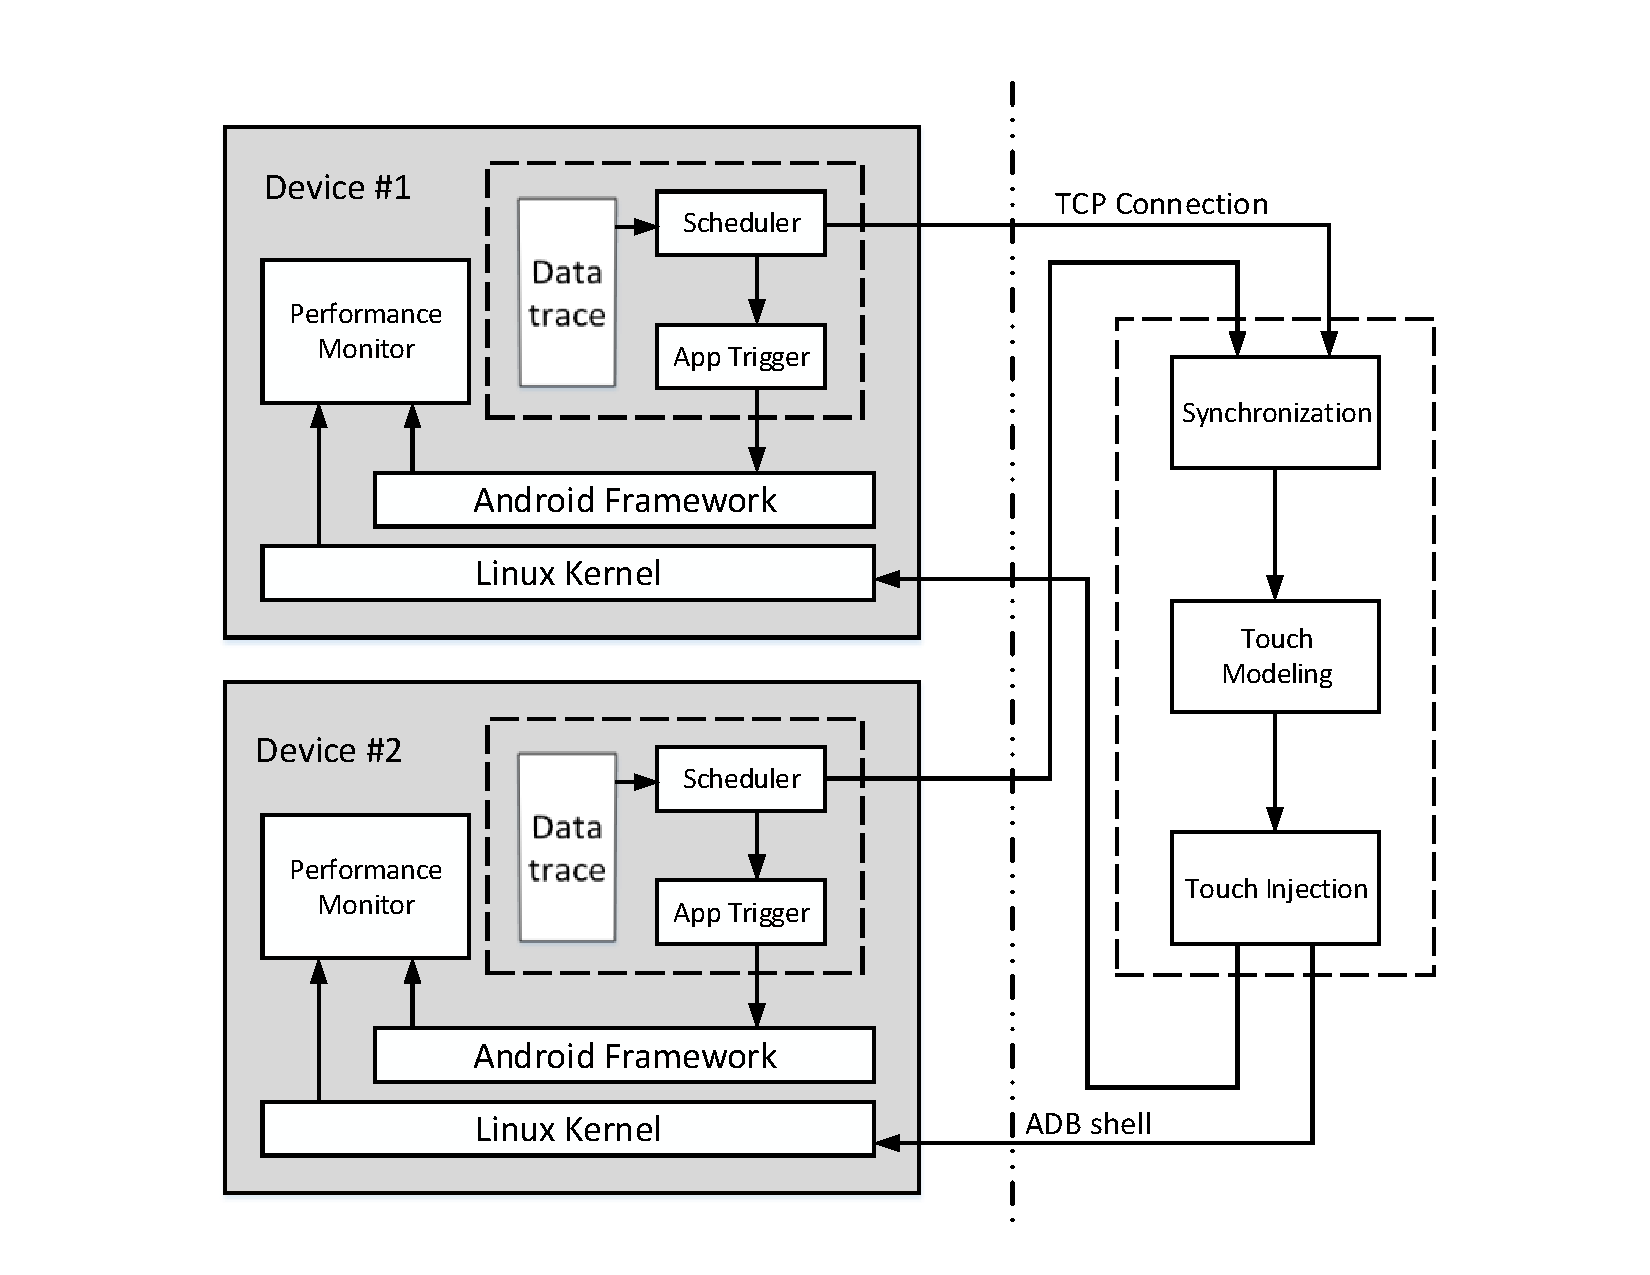
\includegraphics[width=0.45\textwidth]{figures/sys-arch.pdf}
\caption{ReCapture System Architecture}
\label{fig:sys}
\end{figure}

\subsection{Traces and Screen Operations}
As we have discussed, the activity log comes from the existing trace. For example, the \emph{Livelab} data set from Rice University has an app usage trace of $25$ users. The critical information of the data trace includes package name, start time and duration. This three tuple gives the exact running period of an activity event. The package name identify which app and its UI needs to bring to the screen front; the start time gives the relative sequential information of different activity events, which actually is not as important as the package name and the duration; finally the duration specifies how long the app will be use, then the central master will continue issue enough screen actions within the usage period. 

Since the app start timestamp is not as important as the rest two factors, we usually do not need to contain the timestamp information but we require the order of the activity events in the log is first happen first schedule. Then a configurable gap between activity events will be inserted, replacing the original idle period in the data trace. We change the trace in this way simply because we need to shrink the execution time. For instance, the Livelab data trace lasts about one year, but we cannot wait for a year. After we analyze the data set, we find most of the time is idle, so it is safe to replace the large amount of idel period with a fixed gap between activity events.

A sample process is shown in Fig.~\ref{fig:big2}. The central master will take the trace and assign the activity event to different device in time sequence. Thus, each device should have a timeline to trigger the activity event in the smartphone. All devices trigger its own activity event after receiving the activity event from the central master, and the trigger is independent among all devices.

\begin{figure}
\centering
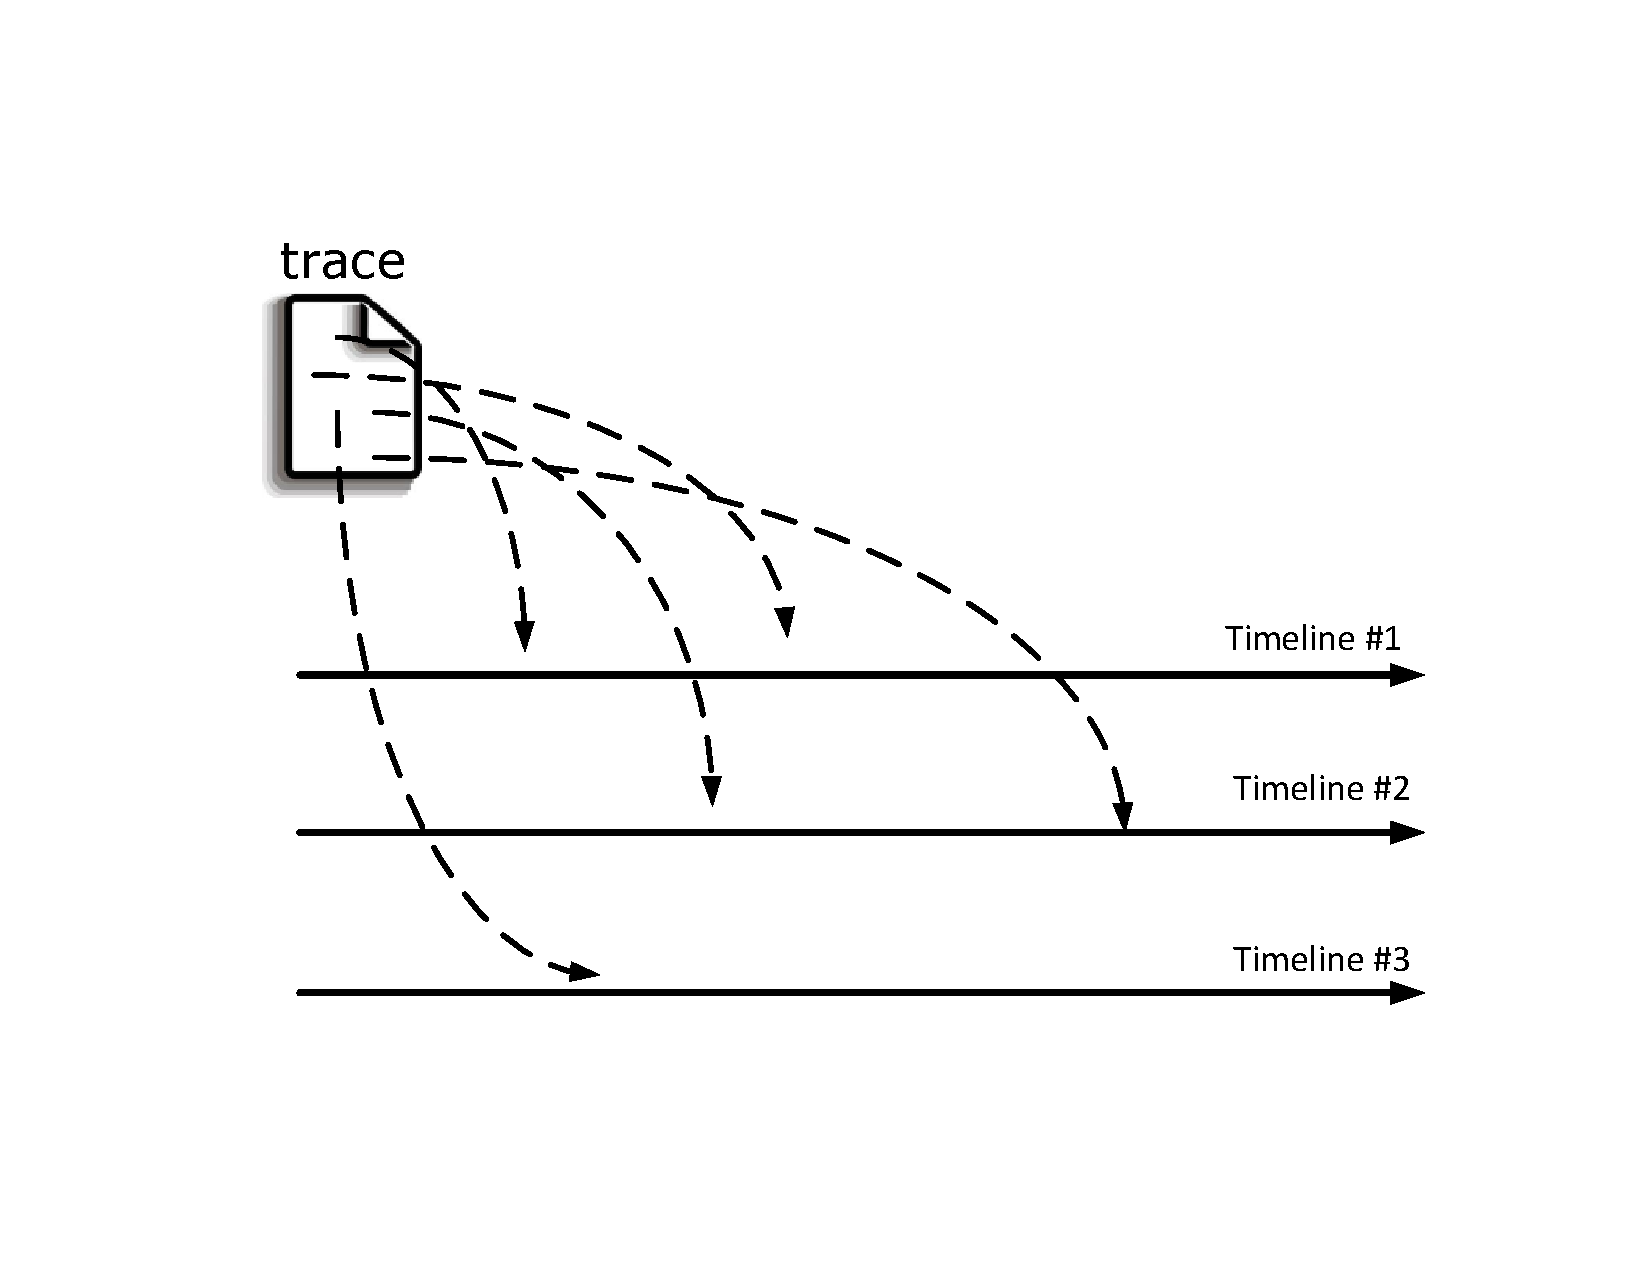
\includegraphics[width=0.45\textwidth]{figures/big-picture2.pdf}
\caption{A sample trace assignment}
\label{fig:big2}
\end{figure}

\subsection{Scalability}
Another important feature in the ReCapture framework is the scalability, which should scale up as many devices as possible at the same time. The reason is obvious that the more devices running simultaneously, the more data we will collect.

Suppose we have unlimited number of physical devices, the scalability is easy to control because we just need to open more USB ports for the extra devices. Unfortunately, the reality is not so convenient in two fold: 1) the number of USB port is not infinite, but our experiment may requires thousands of devices running together; 2) we may only afford less than $10$ devices at a time. Therefore, we need to use an alternative approach to reach the scalability.

Virtualization seems to be the only solution to make the scalability possible and linearly scale up. If we virtualize the physical environment of the smartphone, we may be able to scale $5$ times or more. Existing works have explored the possibility relatively well, so we do not spend too much effort in the virtualization part or scalability issue here.

\section{System Implementation} \label{sec:implementation}
We choose Android OS as the desired smartphone platform for the implementation\footnote{Source code is hosted on Github: https://github.com/little-eyes/ReCapture.git}, and we use several Nexus S smartphones as the hardware. The ReCapture framework is separated into two parts: on-device component and central master component. The existence of on-device component is an Android Service running at the background of the system. It has to be a Service because the screen will be preempted by various different app scheduled by the on-device component.

Specifically, the on-device component has the following Java packages needed in the system:
\begin{itemize}
\item \emph{com.android.recapture.builtin}. This package is the place we used to register and maintain the performance monitor plugin. Each performance monitor module is presented as an Android Service which independently record their metrics. The implementations is different from the all-in-one style because the separate monitor Service gives the developer the largest flexibility to plugin their own metrics.

\item \emph{com.android.recpature.lib}. This library package is the core of the ReCapture framework on each device. It contains critical components in the design diagram, such as \emph{Application Event}, \emph{Application Trigger}, \emph{Emulation Scheduler}, \emph{Activity Hook}. The application event abstract the class of an activity event which contains its corresponding application trigger and activity hook. The application trigger is used to bring the app to the front screen, and the activity hook is used to send a message to the central master where the related screen actions will be issued.

Finally, the emulation scheduler is the central controller in the smartphone where every application event is scheduled one by one for a certain duration. Additionally, the Configuration Manager is the place for the global configuration for the on-device component, where a developer can define the application execution parameters, canonical application name, and data output directory, etc.

\item\emph{com.android.recapture.ui}. This package is mainly about the main entrance of the ReCapture framework. A developer can implement any UI frames in this package if necessary, but we default package do not include any UI framework because the UI activity will be preempted by other apps sooner or later. In addition, the MainService is the main entrace which used to activate the emulation scheduler and other monitor plugins.
\end{itemize}

Note that the activity hook message contains the device's physical ID and current active package. We use the smartphone's device serial number as the physical unique ID because it is identical to the device ID recognized in ADB shell. So we do not need an additional unique ID map from one ID system to another.

On the other hand, the central master component is implemented in the Python. Note that the interactions between the on-device component and the central master are two parts. One is the interaction from the application hook to the central master, which is used to register the current executing app and require the screen actions. Even though the smartphones are connected with the central master with a USB cable, we do not use the standard USB communication at this stage. There are multiple USB connected devices and each device may runs several virtual machines, so the differentiation from USB port to another is complicated. Therefore, we choose a simple TCP connection to bridge the connection from application hook to the central master. Consider the possibility that the two or more screen action requests may come concurrently, the central master's front-end is actually a multi-threaded TCP server which can handle the requests simultaneously.

For the other side of the communication, the central master usually issue the screen actions through the USB cable because this feature requires the Android SDK tool \emph{monkey}'s help. The Android monkey tool provides the ability for the developer to define its own screen action workflow through its script language. A sample language is shown in the Table~\ref{tab:script}. This script's task is to start the \emph{com.android.recapture.ui} package and continuously press different types of keys. Similarly, we the ReCapture framework will prepare each activity event a script based on their usage behavior studies, then the commands will be sent to the device one by one via the USB cable by using ADB commandline automatically.

\begin{table}
\centering
\caption{The sample screen action script}
\begin{tabular}{|l|}\hline
\# Start of Script \\
type= user\\
count= 49\\
speed= 1.0\\
start data $>>$\\
LaunchActivity(com.android.recapture.ui)\\
\# 3120021258\\
DispatchPress(KEYCODE\_3)\\
UserWait(200)\\
DispatchPress(KEYCODE\_1)\\
UserWait(200)\\
DispatchPress(KEYCODE\_3)\\
UserWait(200)\\
DispatchPress(KEYCODE\_5)\\
UserWait(200)\\
DispatchPress(KEYCODE\_0)\\
UserWait(200)\\
DispatchPress(KEYCODE\_2)\\
UserWait(200)\\\hline
\end{tabular}
\label{tab:script}
\end{table}

\section{Preliminary Evaluation}\label{sec:evaluation}
In this section, we discuss some preliminary evaluation results about the ReCapture framework. We use one laptop as the central master of the ReCapture framework and two Google Nexus S smartphones. The Nexus S smartphone's specifications are shown in Table~\ref{tab:nexus}. In addition, Fig.~\ref{fig:exp} displays the experiment environment that two Nexus S smartphones connect to a laptop as the central master.

\begin{table}
\centering
\caption{The Nexus S smartphone specifications}
\begin{tabular}{ll}\toprule
CPU & 1 GHz Cortex-A8 \\
GPU & PowerVR SGX540 \\
RAM & 512MB \\
Storage & 8GB \\
Sensors & Accelerometer, gyro, proximity, compass \\
GPS & Yes, with A-GPS support\\
OS & 4.1.2 (Jelly Bean) \\\bottomrule
\end{tabular}
\label{tab:nexus}
\end{table}

\begin{figure}
\centering
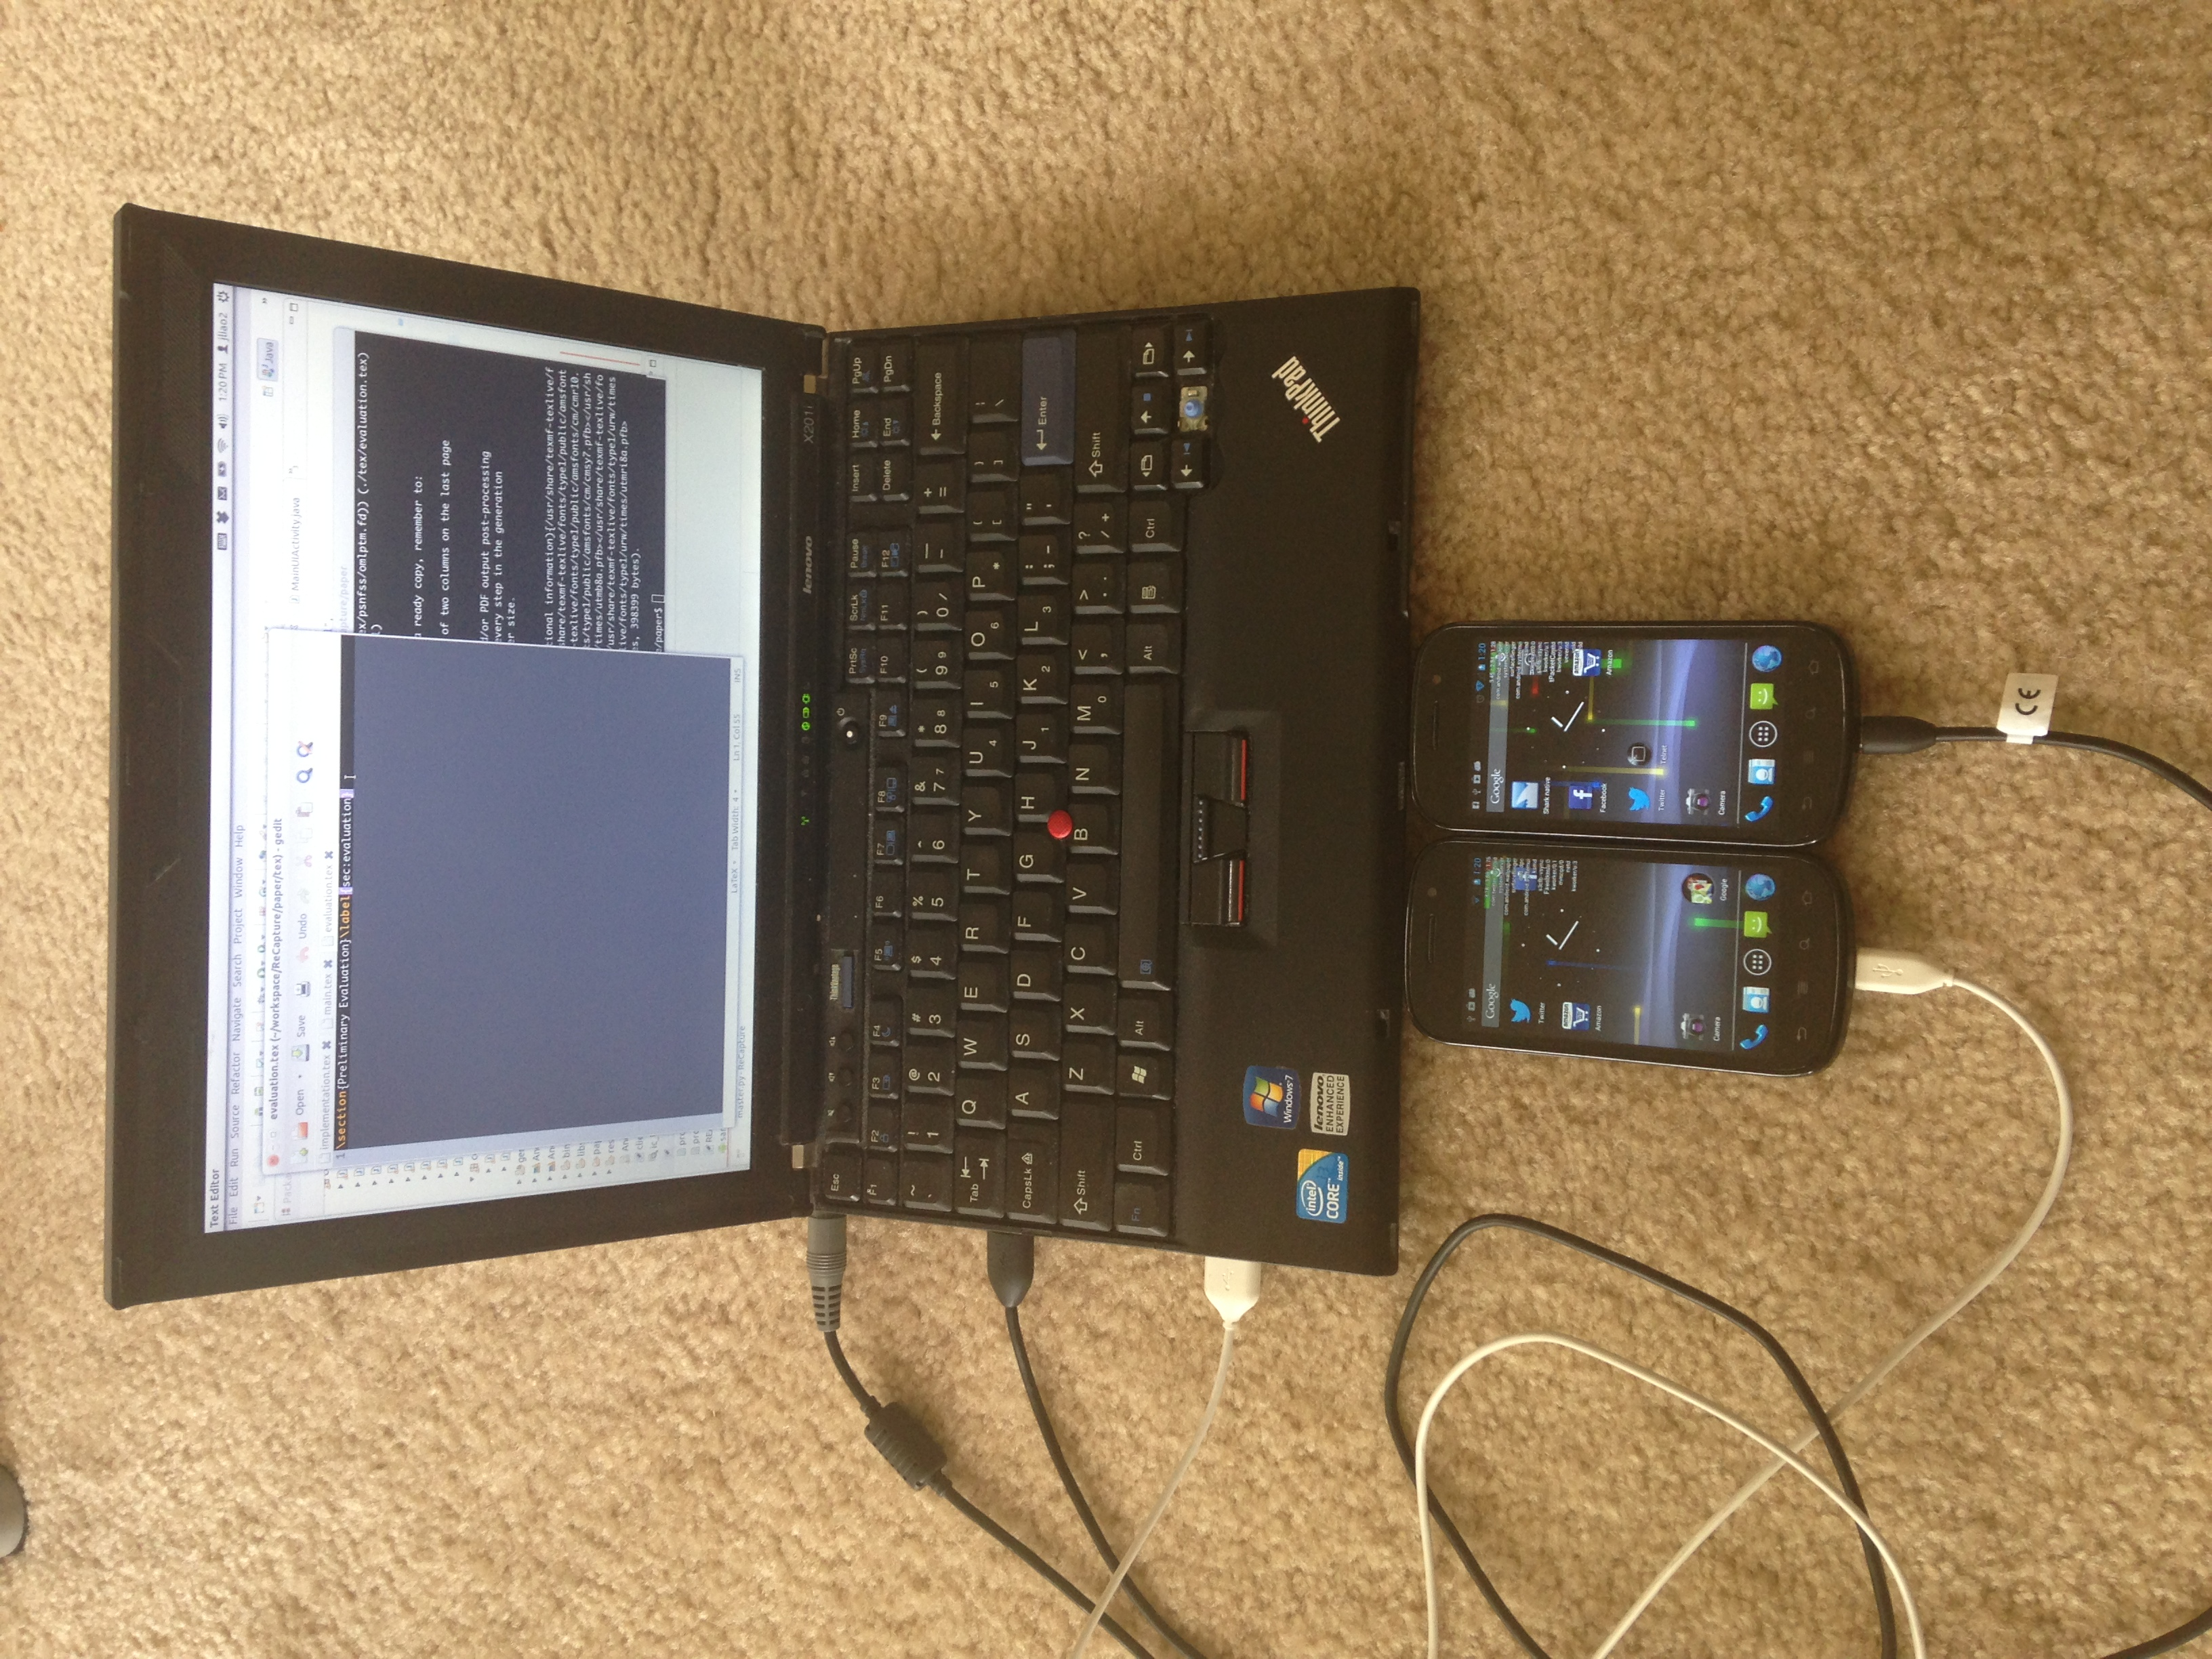
\includegraphics[width=0.45\textwidth]{figures/experiment.jpg}
\caption{Experiment setups}
\label{fig:exp}
\end{figure}

We prepare a sample activity log in the Table~\ref{tab:log}, which we repeat the execution of facebook, gmail, twitter and amazon app and each of the app will last $5$ seconds. After a round of execution, we collect the screen actions issued to the devices and the statistics is shown in Table~\ref{tab:screen}. As we can see, the most active screen operations are navigations, touch and motion. If you are using facebook, you may swipe up and down to see new feeds or use the navigations to jump into to chat. It is also frequent that the you may see a picture and you click the picture, then you change the orientation of the phone to see the picture, so the motions activities also introduces about $10$ percent of the total screen actions. Further more, Fig.~\ref{fig:master} records a screen snapshot of the central master. Once the master receives activity hook message, it will start generate the screen action code to the device.

\begin{figure*}
\centering
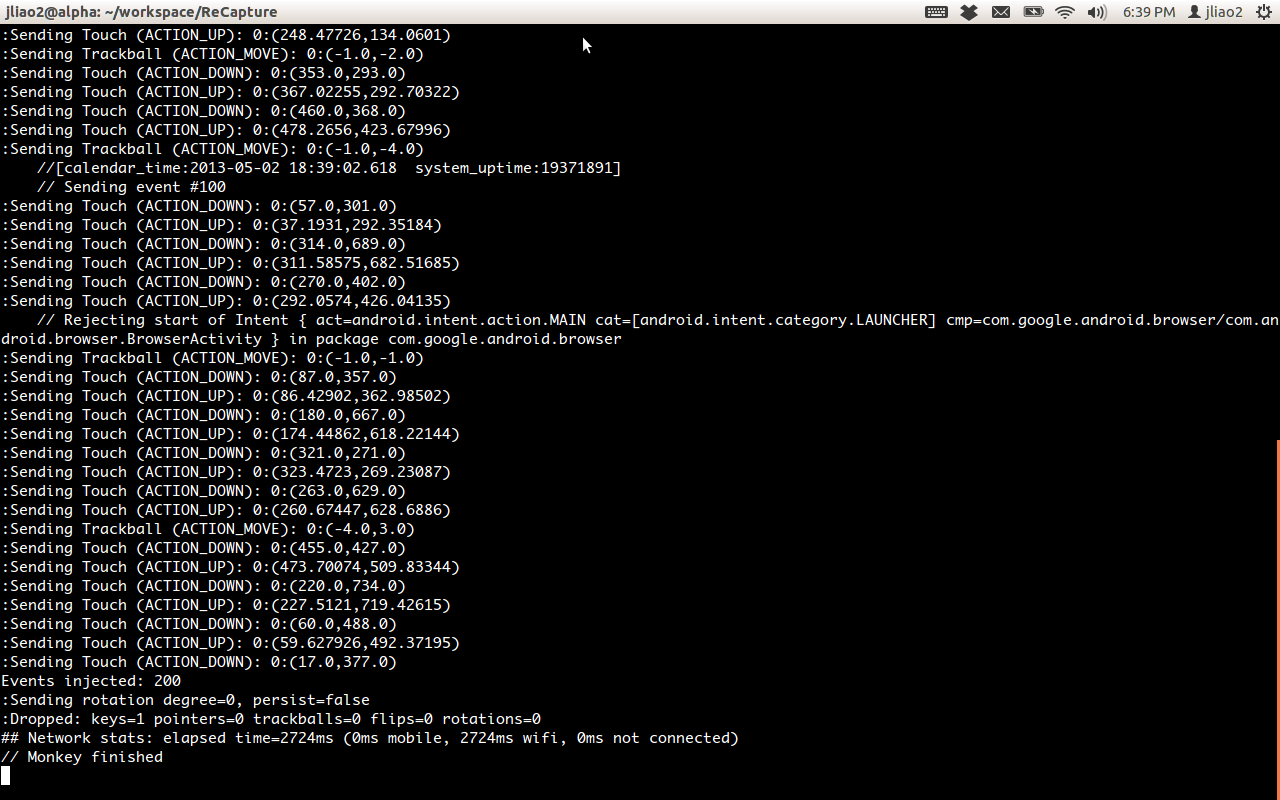
\includegraphics[width=0.8\textwidth]{figures/master.png}
\caption{The central master screen snapshot}
\label{fig:master}
\end{figure*}

\begin{table}
\centering
\caption{The sample activity log}
\begin{tabular}{ll}\toprule
activity event & duration (ms) \\\midrule
facebook & $5,000$ \\
gmail & $5,000$ \\
twitter & $5,000$ \\
amazon & $5,000$\\\bottomrule
\end{tabular}
\label{tab:log}
\end{table}

\begin{table}
\centering
\caption{Screen actions results}
\begin{tabular}{ll} \toprule
Screen Action Category & Percentage \\\midrule
Touch & 15\% \\
Motion & 10\% \\
Traceback & 2\% \\
System Keys & 0\% \\
Navigations & 25\% \\
Major Navigations & 15\% \\
App Switch & 2\%\\
Flip & 2\% \\
Others & 10\% \\\bottomrule
\end{tabular}
\label{tab:screen}
\end{table}

On the other hand, we are interested in the central master's capability to receive large amount of screen action request. It is important because the central master could become the bottleneck of the system in a large scale environment. In this experiment, we test how well the central master can answer the request from the device by sending $1,000,000$ request in multiple thread concurrently to the central master. Fig.~\ref{fig:time} shows the results, as we can see, $90\%$ of the request can get response within $2$ms, so the delay of the system is very small. It is safe to say that the central master should not become a bottleneck of the whole system.

\begin{figure}
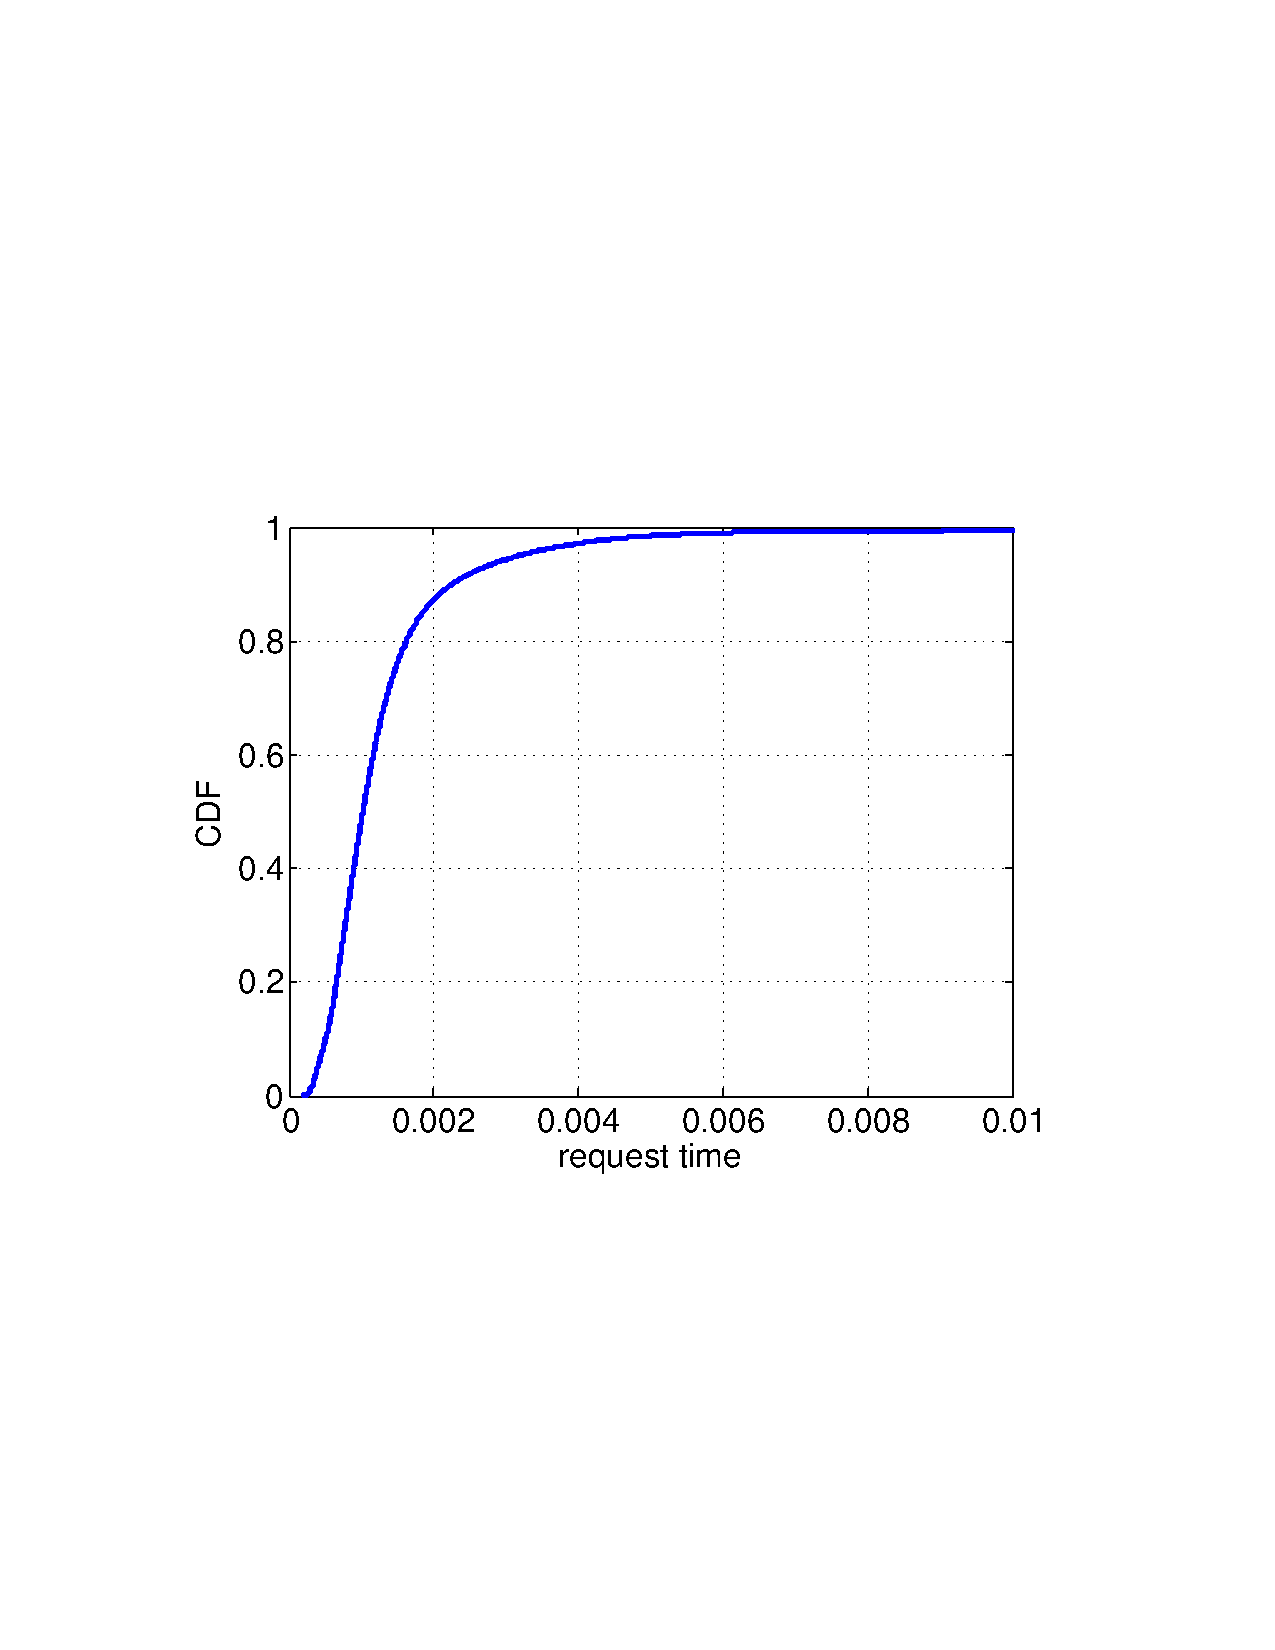
\includegraphics[width=0.45\textwidth]{figures/time.pdf}
\caption{Time response of central master}
\label{fig:time}
\end{figure}

\section{Discussion and Future Work}\label{sec:discussion}
In this section, we discuss some important factors in the system which could be improved through different optimizations.

The first one we are interested in is the system's architecture. As is illustrated in the design section, we separate the system into two parts: on-device part and central master. However, it is possible to move the scheduler into the central master so that the on-device component only contains the performance monitor module. This design makes the architecture on-device very slim and lightweight. We did not design in this way for two reasons: 1) if the testbed is in large scale, or we have the virtual machines runs in the device, centralize the scheduler for all devices will increase the delay a lot. Even though we did not do the relevant experiment, putting thousands of devices' scheduling information into a single place is not an easy task; 2) the distributed design could minimize the cost of single point failure. It is possible the central master could crash, if we put all the scheduling information in the central master, we have to re-do the experiment again if we do not want to lose any information. In contrast, if the scheduler is distributed, the failure cost is only a small portion. Restart the central master, then everything is still on-schedule.

Another issue we think important is the virtualization technology. In Section~\ref{sec:relatedwork} we have discussed some existing work of virtualizing smartphones. Unfortunately, the scalability of virtualization on smartphone is not satisfactory. Usually, two or three virtual phones in one physical phones have reached the limits. In our case, we are caring scalability more than any other factors. Therefore, the existing technology may not be a good fit.

The new approach to make this happen, we believe, could be something more lightweight and should be in higher level, say application level. We think the application itself could be virtualized. First, if we virtualize applications, we need the possibility that two or more apps could run simultaneously while we only have one screen. This problem has been handled very well in Windows 8 operating system which you can run two apps side by side, but we still need more research in the Android system. Second, application vitrualization does not require a whole operating system stack to be virtualized, in which way the extra cost could be minimized.

\section{Conclusion}\label{sec:conclusion}
In this project, we design and implement an automatic evaluation tool and testbed for mobile system. Throughout the design, implementation and evaluation process, we think the ReCapture can now help researchers to evaluate their system work more easily by just configuring the ReCapture framework and let it run. However, the scalability of the ReCapture is linear with the number of devices. We are working on the virtualization technology which could break through the framework's scalability so that ReCapture could serve in large scale evaluation.



{\footnotesize
\bibliographystyle{IEEEtran}
\bibliography{reference}}  % sigproc.bib is the name of the Bibliography in this case

\end{document}


